% !TEX root = main.tex
% ══════════════════════════════════════════════════════════════
\section{Introdução}
% ══════════════════════════════════════════════════════════════

A robótica móvel tem experimentado um crescimento sem precedentes nas últimas décadas, deixando de ser um campo puramente experimental para se tornar uma solução prática em setores como logística, saúde e serviços domésticos. Segundo \cite{pendleton2017}, o sucesso de um sistema autônomo está intrinsecamente ligado à sua capacidade de fechar o ciclo entre percepção, planejamento e controle. Para que um robô opere de forma segura em ambientes compartilhados com seres humanos, ele precisa processar fluxos massivos de dados sensoriais e transformá-los em decisões motoras em milissegundos.

Dentro deste vasto campo, os robôs seguidores (\textit{follow-me robots}) representam um desafio de engenharia particularmente interessante. Diferente de robôs de navegação global que seguem rotas pré-definidas por GPS ou mapas estáticos, o robô seguidor deve lidar com um alvo dinâmico e, muitas vezes, imprevisível. De acordo com \cite{quigley2015programming}, a modularidade proporcionada pelo \textit{Robot Operating System} (ROS) é o que permite que desenvolvedores integrem algoritmos complexos de visão e laser de forma eficiente, facilitando a criação de comportamentos reativos como o rastreamento de alvos.

O desafio central da percepção robusta reside nas limitações intrínsecas de cada sensor quando utilizados de forma isolada. Câmeras RGB, embora forneçam dados semânticos valiosos sobre cor e textura, carecem de precisão na medição de profundidade. Conforme discutido por \cite{zhang2019robust}, a fusão sensorial surge como a solução para este dilema. Ao combinar a capacidade de identificação da câmera com a precisão métrica do LiDAR, é possível mitigar falhas causadas por variações de iluminação ou oclusões parciais, problemas comuns em cenários reais de operação.

Neste trabalho, utiliza-se a plataforma robótica Agilex LIMO \cite{agilex2024limo}, um robô compacto e versátil equipado com múltiplos sensores, para implementar e validar um sistema de seguimento baseado em fusão de dados. O projeto evolui de uma primeira abordagem baseada em detecção de alvo por cor no espaço HSV para uma segunda abordagem baseada em detecção de objetos por categoria com a rede neural YOLO, incorporando ainda campos potenciais para aproximação segura e desvio de obstáculos.

\subsection{Objetivos}

O objetivo principal desta pesquisa é desenvolver, implementar e testar um pipeline de software capaz de transformar o robô LIMO em um sistema autônomo de seguimento. Para alcançar este objetivo geral, definem-se os seguintes objetivos específicos:
\begin{itemize}
    \item Desenvolver um nó de processamento visual para detecção de alvos coloridos robusto a ruídos;
    \item Implementar a leitura sincronizada do sensor LiDAR para extração de distâncias em ângulos específicos;
    \item Criar um algoritmo de fusão que unifique as coordenadas da câmera e do laser;
    \item Projetar um controlador proporcional para velocidades lineares e angulares;
    \item Implementar um comportamento de busca ativa (rotação 360°) para recuperação do alvo em caso de perda de detecção;
    \item Estender o sistema com detecção de objetos por categoria usando a rede YOLO e uma estratégia de aproximação baseada em campos potenciais com freio de segurança.
\end{itemize}

\subsection{Justificativa}

A escolha pela integração entre câmera e LiDAR justifica-se pela busca por redundância e confiabilidade. Enquanto a câmera atua como o "olho" que identifica a natureza do objeto, o LiDAR funciona como o "tato" que define a geometria do ambiente ao redor. Conforme sugerido por \cite{nguyen2020lidar}, sistemas que utilizam LiDAR apresentam uma taxa de sucesso significativamente maior em evitar colisões em ambientes dinâmicos. Portanto, a fusão proposta não apenas melhora a qualidade do seguimento, mas eleva o padrão de segurança operacional do robô em proximidade com obstáculos ou pessoas.


% ══════════════════════════════════════════════════════════════
\newpage
\section{Revisão Bibliográfica}
% ══════════════════════════════════════════════════════════════

% --------------------------------------------------------------
\subsection{Veículo Autônomo LIMO AgileX}
% --------------------------------------------------------------

O LIMO é uma plataforma robótica móvel compacta desenvolvida pela AgileX
Robotics, projetada para pesquisa e ensino em robótica móvel~\cite{pimenta2024limo}.
Apesar do porte reduzido — ideal para espaços de trabalho limitados —, o robô é
equipado com sensores e capacidade computacional suficientes para estudos de
navegação autônoma, SLAM, mapeamento, planejamento de trajetórias e desvio de
obstáculos. A Figura~\ref{fig:limo_pro} mostra o modelo LIMO Pro utilizado neste
trabalho.

\begin{figure}[H]
  \centering
  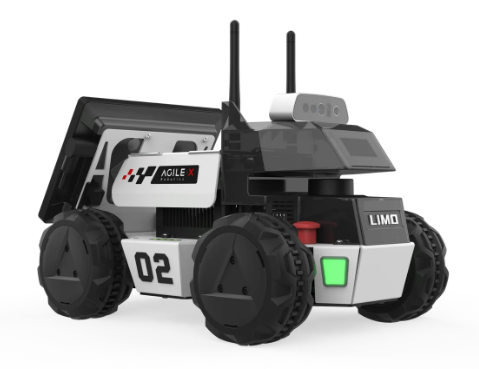
\includegraphics[width=0.5\textwidth]{images/tg1/introducao/limo_pro.png}
  \caption{LIMO Pro da AgileX Robotics.}
  \label{fig:limo_pro}
\end{figure}

\subsubsection{Modos de Operação}

Uma característica distintiva do LIMO é sua capacidade de assumir quatro
configurações cinemáticas diferentes, selecionáveis mecanicamente por travas na
parte frontal do chassi~\cite{pimenta2024limo}:

\begin{itemize}
  \item \textbf{Diferencial}: quatro rodas em que as duas de um mesmo lado são
  acionadas em conjunto; a diferença de velocidade entre os lados produz rotação.
  \item \textbf{Esteira}: sobrepõem-se esteiras às rodas, oferecendo maior tração
  e estabilidade em terrenos irregulares; é controlado como o modo diferencial.
  \item \textbf{Omnidirecional}: com rodas Mecanum, permite deslocamentos
  longitudinais e laterais independentes da orientação do robô.
  \item \textbf{Ackermann}: direção do tipo automóvel, adequada à validação de
  algoritmos para veículos não-holonômicos.
\end{itemize}

Neste trabalho o robô é utilizado na configuração \textbf{diferencial}. Nesse
modo, as velocidades linear $v$ e angular $\omega$ do robô relacionam-se com as
velocidades angulares das rodas esquerda ($\omega_L$) e direita ($\omega_R$)
por~\cite{pimenta2024limo}:

\begin{equation}
  \label{eq:cinematica}
  v = \frac{(\omega_L + \omega_R)\, r_w}{2}, \qquad
  \omega = \frac{(\omega_R - \omega_L)\, r_w}{b},
\end{equation}

onde $r_w$ é o raio da roda e $b$ a distância entre as rodas de lados opostos. O
controlador de baixo nível embarcado no LIMO converte automaticamente os comandos
de alto nível $u = [\,v \;\; \omega\,]^T$ — publicados no tópico \texttt{/cmd\_vel}
— nos sinais PWM enviados aos motores, de modo que o desenvolvedor trabalha
diretamente no nível das velocidades linear e angular.

\subsubsection{Computador de Bordo e Software}

O processamento embarcado é realizado por uma placa \textbf{NVIDIA Jetson Nano},
que integra uma CPU quad-core ARM Cortex-A57 de 64 bits a 1,43~GHz, 4~GB de
memória RAM LPDDR4 e uma GPU Maxwell de 128 núcleos com suporte a aceleração de
aprendizado profundo~\cite{pimenta2024limo}. Essa GPU é o que viabiliza a
execução de redes neurais de detecção, como o YOLO, diretamente a bordo do robô.
A alimentação é feita por uma bateria de 12~V e 5200~mAh, com autonomia de
aproximadamente 40 minutos em operação ativa. O robô conta ainda com uma unidade
de medição inercial (IMU) de 6 graus de liberdade e um chassi metálico de cerca
de 4,8~kg que suporta até 4~kg de carga útil.

Em software, a Jetson Nano executa \textbf{Ubuntu 18.04} com o SDK NVIDIA
JetPack. O driver do robô é fornecido pela AgileX como um pacote ROS
(\texttt{limo\_base}), responsável pela comunicação com o chassi, pela publicação
da odometria e pela recepção dos comandos de velocidade. O pacote
\texttt{limo\_bringup} reúne os \textit{launchers} que inicializam o driver, o
LiDAR e a árvore de transformadas (\textit{tf}) entre a base, a câmera, a IMU e o
laser~\cite{pimenta2024limo}.

\subsubsection{LiDAR — EAI T-Mini Pro}

O sensor LiDAR utilizado é o \textbf{EAI T-Mini Pro (YDLidar)}, que realiza
varreduras angulares do ambiente emitindo feixes de laser e medindo o tempo de
retorno de cada pulso. O resultado é um conjunto de pares $(\theta, d)$, onde
$\theta$ é o ângulo e $d$ é a distância até o obstáculo mais próximo naquela
direção, formando um mapa de pontos 2D do ambiente.

As principais características relevantes para este projeto são:

\begin{itemize}
  \item Ângulo de varredura: $-90°$ a $+90°$ (frontal)
  \item Frequência de atualização: $\approx 9$ Hz
  \item Distância mínima: $0{,}15$ m
  \item Distância máxima: $12$ m
\end{itemize}

As Figuras~\ref{fig:corredor} e~\ref{fig:lab} mostram mapas de pontos gerados
pelo LiDAR em diferentes ambientes.

\begin{figure}[H]
  \centering
  \begin{subfigure}[b]{0.48\textwidth}
    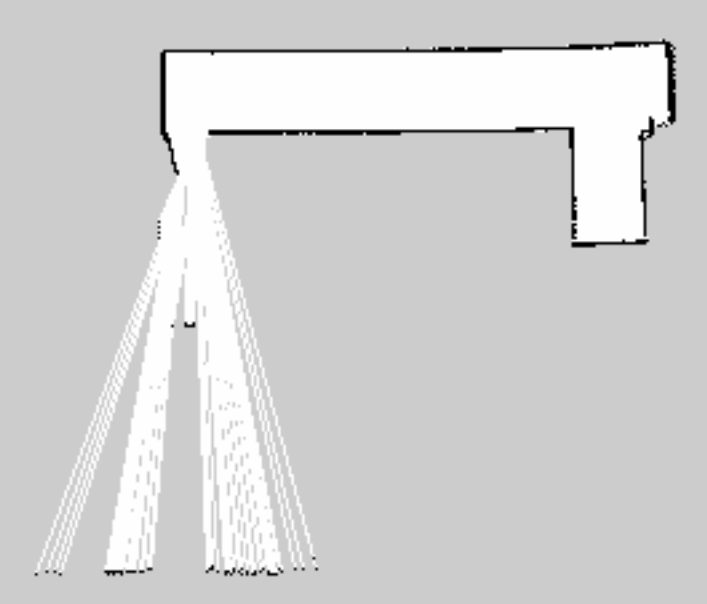
\includegraphics[width=\textwidth]{images/tg2/corredorzinho.png}
    \caption{Mapa de pontos — corredor}
    \label{fig:corredor}
  \end{subfigure}
  \hfill
  \begin{subfigure}[b]{0.48\textwidth}
    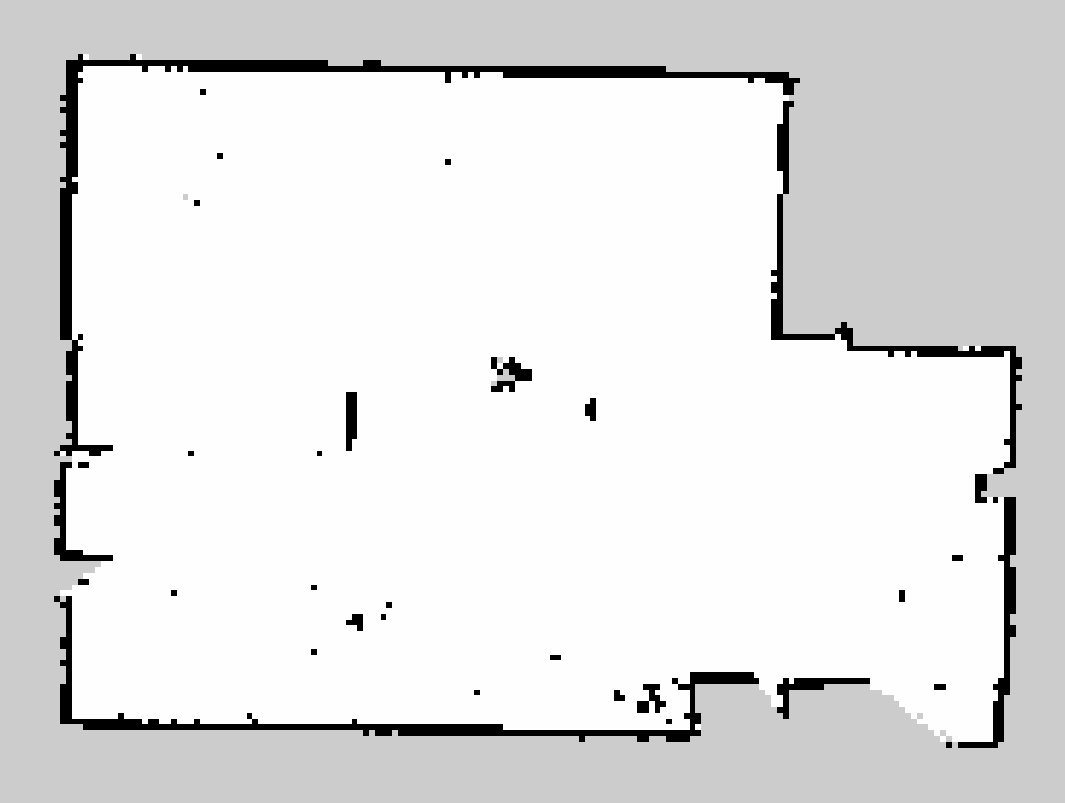
\includegraphics[width=\textwidth]{images/tg2/lab_LEVE.png}
    \caption{Mapa de pontos — laboratório}
    \label{fig:lab}
  \end{subfigure}
  \caption{Varreduras do LiDAR EAI T-Mini Pro em diferentes ambientes.}
\end{figure}

\subsubsection{Câmera — Orbbec Astra (Dabai U3)}

A câmera utilizada é a \textbf{Orbbec Astra Dabai U3}, uma câmera RGB-D
(colorida com profundidade) com campo de visão horizontal de $60°$ e resolução
de $640 \times 480$ pixels a 30 fps. Neste projeto é utilizado apenas o canal
RGB, publicado no tópico \texttt{/camera/rgb/image\_raw}. A figura~\ref{fig:teste_camera} mostra o tópico sendo monitorado via Foxglove Studio durante os testes.

\begin{figure}[H]
  \centering
  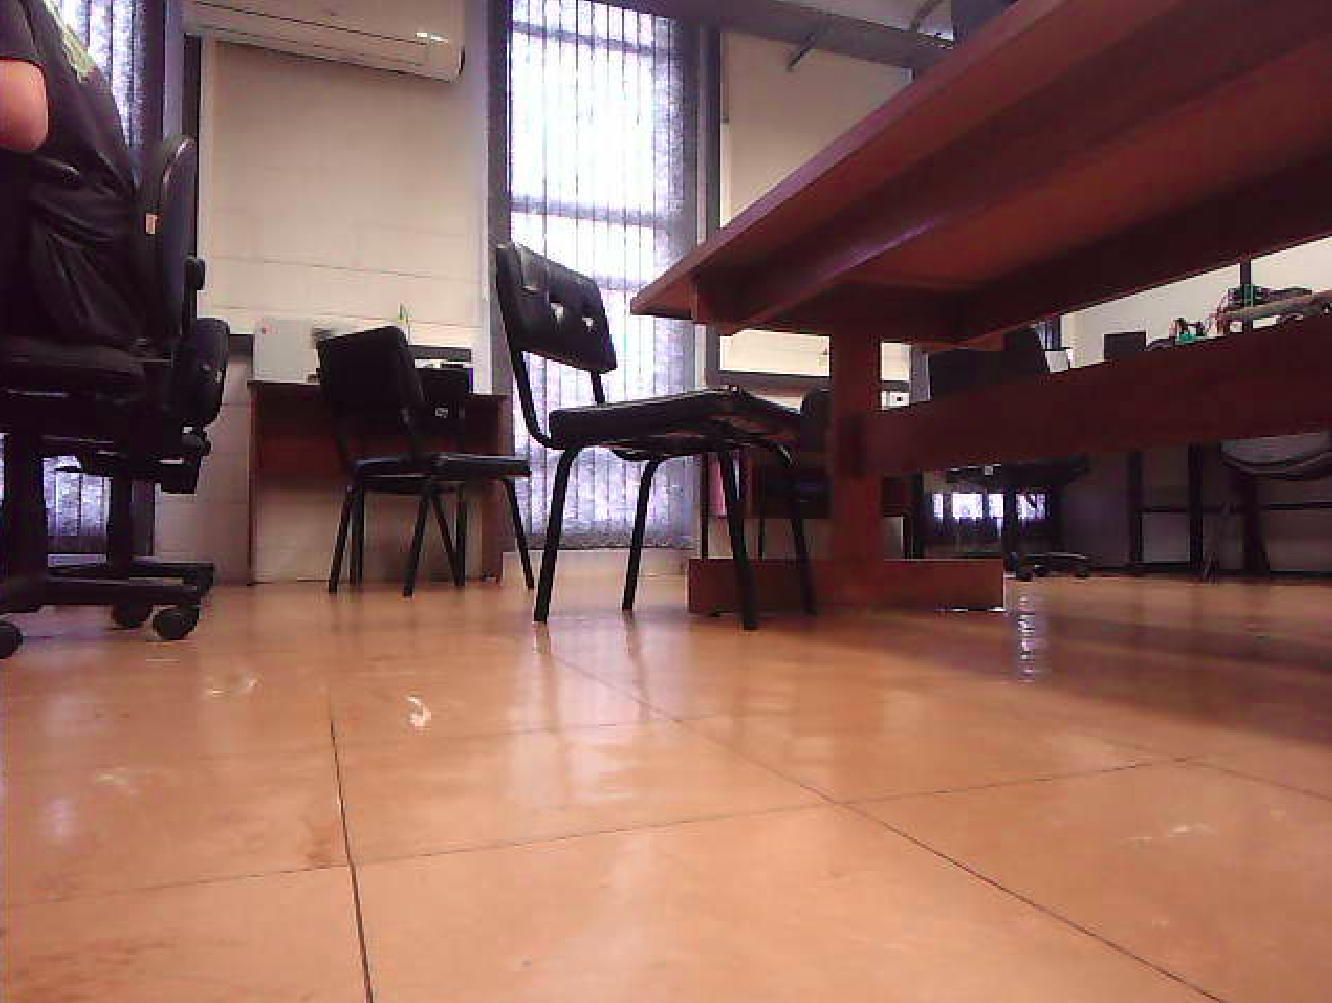
\includegraphics[width=0.7\textwidth]{images/tg2/teste_camera.png}
  \caption{Visualização do tópico /camera/rgb/image\_raw no Foxglove Studio.}
  \label{fig:teste_camera}
\end{figure}

% --------------------------------------------------------------
\subsection{Robot Operating System (ROS)}
% --------------------------------------------------------------

O Robot Operating System (ROS) é um arcabouço de software (\textit{framework})
de código aberto voltado ao desenvolvimento de aplicações
robóticas~\cite{quigley2009ros}. Apesar do nome, não se trata de um sistema
operacional convencional, mas de um \textit{meta}-sistema operacional que roda
sobre o Linux e provê os serviços que se esperaria de um sistema operacional no
contexto da robótica: abstração de \textit{hardware}, controle de dispositivos em
baixo nível, troca de mensagens entre processos e gerenciamento de pacotes, além
de um conjunto de ferramentas e bibliotecas para obtenção, compilação e execução
de código distribuído entre múltiplos computadores~\cite{quigley2015programming}.

A principal motivação do ROS é facilitar a integração e o reúso de software em
robótica. Em vez de um único programa monolítico, o sistema é decomposto em vários
blocos independentes — os \textbf{nós} (\textit{nodes}) —, cada um responsável por
uma tarefa pequena e bem definida, como a aquisição de dados de um sensor, uma
malha de controle ou o acionamento de um atuador. Essa modularidade permite
desenvolver, testar e substituir cada componente isoladamente, característica
diretamente explorada neste trabalho, no qual cada etapa do \textit{pipeline} é
implementada como um nó separado.

Neste projeto é utilizado o \textbf{ROS 1 Melodic}, rodando sobre Ubuntu 18.04 no
\textit{hardware} embarcado (NVIDIA Jetson Nano) do LIMO.

\subsubsection{Arquitetura \textit{Publish-Subscribe}}

A comunicação entre os nós segue majoritariamente o padrão
\textit{publish-subscribe}. Um nó \textbf{publica} (\textit{publisher}) mensagens
em um \textbf{tópico} nomeado, e qualquer outro nó interessado pode \textbf{assinar}
(\textit{subscriber}) esse tópico para recebê-las, sem que haja acoplamento direto
entre eles: o publicador não sabe quais nós são os assinantes, e vice-versa. Esse
desacoplamento é o que confere flexibilidade ao sistema — foi ele, por exemplo,
que permitiu reaproveitar o nó \texttt{lidar\_reader} no modo de tarefas apenas
remapeando o tópico de entrada, sem alterar seu código.

O registro e a descoberta dos nós e tópicos são coordenados por um processo mestre,
o \textbf{\texttt{roscore}} (ROS \textit{Master}). É ele quem permite que um
publicador e um assinante se localizem; após esse contato inicial, a troca de
mensagens ocorre diretamente entre os nós. A Figura~\ref{fig:pubsub} ilustra o
conceito.

\begin{figure}[H]
\centering
\begin{tikzpicture}[
  node distance=1.4cm and 2.0cm,
  box/.style={rectangle, rounded corners, draw=blue!40, fill=blue!10,
              minimum width=2.3cm, minimum height=0.9cm, align=center, font=\small},
  master/.style={rectangle, rounded corners, draw=green!45, fill=green!12,
              minimum width=2.3cm, minimum height=0.9cm, align=center, font=\small},
  topic/.style={rectangle, draw=gray!70, fill=gray!12,
              minimum width=2.0cm, minimum height=0.8cm, font=\ttfamily\small},
  arr/.style={-{Stealth}, thick, gray},
  reg/.style={dashed, gray, -{Stealth}}
]
\node[master] (master) {\texttt{roscore}\\(\textit{Master})};
\node[box, below=1.4cm of master, xshift=-3.4cm] (pub) {Nó\\publicador};
\node[topic, below=1.5cm of master] (topic) {/tópico};
\node[box, below=1.4cm of master, xshift=3.4cm] (sub) {Nó\\assinante};

\draw[arr] (pub) -- node[above, font=\scriptsize]{publica} (topic);
\draw[arr] (topic) -- node[above, font=\scriptsize]{assina} (sub);
\draw[reg] (pub) -- node[sloped, above, font=\scriptsize]{registro} (master);
\draw[reg] (sub) -- node[sloped, above, font=\scriptsize]{registro} (master);
\end{tikzpicture}
\caption{Padrão \textit{publish-subscribe} do ROS: o \texttt{roscore} coordena o
registro dos nós (linhas tracejadas) e as mensagens trafegam pelo tópico do
publicador ao assinante (linhas cheias).}
\label{fig:pubsub}
\end{figure}

\subsubsection{Conceitos Fundamentais}

Os principais conceitos do ROS utilizados neste trabalho são:

\begin{itemize}
  \item \textbf{Nós (\textit{Nodes})}: processos independentes, cada um
  responsável por uma tarefa específica. Neste projeto, cada etapa do
  \textit{pipeline} (detecção, leitura do LiDAR, fusão, controle) é um nó separado.

  \item \textbf{Tópicos (\textit{Topics})}: canais de comunicação assíncronos
  pelos quais os nós trocam mensagens, no padrão \textit{publish-subscribe}.

  \item \textbf{Mensagens (\textit{Messages})}: estruturas de dados tipadas que
  trafegam pelos tópicos. Exemplos usados neste projeto:
  \texttt{sensor\_msgs/LaserScan} para dados do LiDAR, \texttt{sensor\_msgs/Image}
  para \textit{frames} da câmera e \texttt{geometry\_msgs/Twist} para comandos de
  velocidade.

  \item \textbf{\textit{Master} (\texttt{roscore})}: processo central que registra
  nós e tópicos e viabiliza que publicadores e assinantes se encontrem.

  \item \textbf{Pacotes (\textit{Packages})}: unidade de organização do código,
  reunindo nós, bibliotecas, arquivos de configuração e \textit{launchers}. Todo o
  código deste trabalho está organizado no pacote \texttt{follower\_limo}.
\end{itemize}

\subsubsection{Ferramentas Utilizadas}

O ROS oferece um conjunto de utilitários de linha de comando que apoiam o
desenvolvimento e a depuração. Os mais utilizados neste trabalho foram: o
\texttt{roscore}, que inicia o \textit{Master}; o \texttt{rosrun} e o
\texttt{roslaunch}, que executam nós individualmente ou em conjunto a partir de
arquivos \texttt{.launch}; e o \texttt{rostopic}, que permite inspecionar,
publicar e medir a frequência das mensagens em um tópico. A visualização dos dados
em tempo real — imagens da câmera, detecções e varreduras do LiDAR — foi feita com
o Foxglove Studio, conectado ao ROS por meio do \texttt{foxglove\_bridge}.

% --------------------------------------------------------------
\subsection{Detecção por Cor (HSV) e Fusão Sensorial}
\label{sec:hsv_fusao}
% --------------------------------------------------------------

\subsubsection{Espaço de Cor HSV}

A primeira abordagem de percepção deste trabalho baseia-se na segmentação por
cor. Embora as câmeras forneçam a imagem no espaço RGB (ou BGR, no OpenCV), esse
espaço mistura, em seus três canais, tanto a informação cromática quanto a
luminosidade, o que o torna sensível a variações de iluminação. Por esse motivo,
adota-se o espaço \textbf{HSV} (\textit{Hue, Saturation, Value}), que
separa a cor em três componentes com significado
perceptual~\cite{gonzalez2018digital}:

\begin{itemize}
  \item \textbf{Matiz (\textit{Hue})}: o tom da cor, representado como um ângulo
  no círculo cromático ($0°$ a $360°$);
  \item \textbf{Saturação (\textit{Saturation})}: a pureza ou intensidade da cor;
  \item \textbf{Valor (\textit{Value})}: o brilho.
\end{itemize}

A vantagem prática é que a identidade cromática de um objeto concentra-se
principalmente no canal de matiz, relativamente independente do brilho. Assim, a
segmentação torna-se mais robusta a mudanças de iluminação do que seria no espaço
RGB. A detecção consiste em construir uma máscara binária $M(x,y)$ que isola os
\textit{pixels} cujos valores caem dentro de faixas pré-definidas:

\begin{equation}
  \label{eq:hsv}
  M(x,y) =
  \begin{cases}
    1, & \text{se } H_{\min} \le H \le H_{\max} \;\wedge\; S_{\min} \le S \le S_{\max} \;\wedge\; V_{\min} \le V \le V_{\max}, \\
    0, & \text{caso contrário}.
  \end{cases}
\end{equation}

Cores que cruzam a origem do círculo de matiz — como o vermelho, situado
simultaneamente próximo a $0°$ e a $360°$ — exigem duas faixas de matiz
combinadas. Após a limiarização, operações morfológicas removem ruído e o maior
contorno válido é tomado como o alvo. Os detalhes de implementação deste processo
são apresentados na Seção~\ref{sec:modo1}.

\subsubsection{Fusão Sensorial}

A detecção por cor localiza o alvo \textit{angularmente} na imagem, mas não
informa a que \textit{distância} ele está. Câmeras RGB, isoladamente, carecem de
precisão métrica de profundidade; o LiDAR, por outro lado, mede distâncias com
exatidão, mas não distingue a natureza ou a cor dos objetos. A
\textbf{fusão sensorial} combina essas modalidades complementares para obter uma
estimativa mais completa e confiável do que qualquer sensor forneceria
sozinho~\cite{zhang2019robust}.

A literatura costuma classificar a fusão em três níveis: no nível de dados brutos,
no nível de características (\textit{feature-level}) e no nível de decisão. Neste
trabalho emprega-se a fusão em \textbf{nível de características}: extrai-se o
ângulo do alvo a partir da câmera e a distância a partir do LiDAR naquela mesma
direção, unindo-os em uma estimativa geométrica única da posição relativa do
alvo. Para atenuar ruídos e saltos nas leituras, aplica-se ainda um filtro de
suavização exponencial, detalhado na Seção~\ref{sec:modo1}. Essa estratégia de
redundância eleva a robustez do sistema: falhas momentâneas de um sensor — como
uma oclusão parcial ou uma variação brusca de iluminação — são mitigadas pela
informação do outro~\cite{nguyen2020lidar}.

% --------------------------------------------------------------
\subsection{YOLO}
% --------------------------------------------------------------

A detecção de objetos é a tarefa de visão computacional que busca responder a duas
perguntas sobre uma imagem: \textit{quais} objetos existem e \textit{onde} eles
estão localizados~\cite{zou2023survey}. O YOLO (\textit{You Only Look Once}) é um
algoritmo de detecção de objetos baseado em aprendizado profundo, proposto
originalmente por~\cite{redmon2016yolo}. Sua
principal inovação foi tratar a detecção como um único problema de regressão,
resolvido por uma única rede neural convolucional que, em uma só passagem
(\textit{single-stage}), prevê simultaneamente as caixas delimitadoras
(\textit{bounding boxes}) e as classes dos objetos presentes na imagem. Essa
abordagem contrasta com os detectores de dois estágios da família R-CNN, que
primeiro geram regiões candidatas e só depois as classificam, sendo
significativamente mais lentos. Por unificar as duas etapas, o YOLO alcança
desempenho em tempo real, característica essencial para aplicações robóticas
embarcadas.

\subsubsection{Divisão em Grade e Predições}

O YOLO divide a imagem de entrada em uma grade de $S \times S$ células. Cada
célula é responsável por detectar objetos cujo centro recai sobre ela, prevendo
$B$ caixas delimitadoras e uma pontuação de confiança para cada uma. Cada caixa é
descrita por cinco valores: as coordenadas do centro e as dimensões
$(x, y, w, h)$ e a confiança associada.

A pontuação de confiança reflete tanto a probabilidade de a caixa conter de fato
um objeto quanto a precisão geométrica da predição, sendo definida como:

\begin{equation}
  \label{eq:confianca}
  \text{Confiança} = \Pr(\text{Objeto}) \cdot \text{IoU}^{\text{verdade}}_{\text{predição}} ,
\end{equation}

onde $\Pr(\text{Objeto}) \in \{0, 1\}$ indica a existência de um objeto na célula
e a IoU (\textit{Intersection over Union}) mede a sobreposição entre a caixa
prevista $B_p$ e a caixa de referência $B_v$:

\begin{equation}
  \label{eq:iou}
  \text{IoU} = \frac{\text{área}(B_p \cap B_v)}{\text{área}(B_p \cup B_v)} .
\end{equation}

Além das caixas, cada célula prevê $C$ probabilidades condicionais de classe,
$\Pr(\text{Classe}_i \mid \text{Objeto})$. No momento da inferência, a
probabilidade condicional é multiplicada pela confiança da caixa, produzindo uma
pontuação específica por classe que combina a probabilidade da classe com a
qualidade do ajuste da caixa:

\begin{equation}
  \Pr(\text{Classe}_i \mid \text{Objeto}) \cdot \Pr(\text{Objeto}) \cdot
  \text{IoU}^{\text{verdade}}_{\text{predição}} =
  \Pr(\text{Classe}_i) \cdot \text{IoU}^{\text{verdade}}_{\text{predição}} .
\end{equation}

O resultado é codificado em um tensor de saída de dimensão:

\begin{equation}
  \label{eq:tensor}
  S \times S \times (B \cdot 5 + C) .
\end{equation}

A título de exemplo, na formulação original com $S = 7$, $B = 2$ e $C = 20$
classes, obtém-se um tensor $7 \times 7 \times 30$.

\subsubsection{Arquitetura}

A arquitetura do YOLO pode ser dividida em três componentes
principais~\cite{ali2024yolo}:

\begin{itemize}
  \item \textbf{\textit{Backbone}}: rede convolucional que extrai características
  (\textit{features}) da imagem em múltiplas escalas, empilhando camadas
  convolucionais.
  \item \textbf{\textit{Neck}}: processa e combina os mapas de características de
  diferentes níveis, garantindo informação multi-escala.
  \item \textbf{\textit{Head}}: a partir das características fundidas, prevê as
  caixas delimitadoras e as probabilidades de classe. A versão YOLOv3 introduziu
  o uso de \textit{anchor boxes} em múltiplas escalas na \textit{head},
  melhorando a detecção de objetos de tamanhos variados~\cite{jiang2022yolo}.
\end{itemize}

O algoritmo possui duas variantes básicas: o modelo completo (\textit{Regular})
e o modelo reduzido (\textit{Tiny}). Enquanto o modelo completo do YOLO original
emprega 24 camadas convolucionais seguidas de 2 camadas totalmente conectadas, a
versão \textit{Tiny} utiliza um número muito menor de camadas, sacrificando parte
da precisão em troca de uma inferência consideravelmente mais rápida e de menor
custo computacional. Essa característica torna a versão \textit{Tiny} adequada a
plataformas embarcadas com recursos limitados, como a Jetson Nano do LIMO.

\subsubsection{Supressão Não-Máxima (NMS)}

Como várias células podem prever caixas para um mesmo objeto, gera-se um conjunto
redundante de detecções. Para produzir uma saída limpa, aplica-se a supressão
não-máxima (\textit{Non-Maximum Suppression}, NMS): as caixas são ordenadas por
confiança e, iterativamente, mantém-se a de maior pontuação enquanto se descartam
as demais que apresentem IoU acima de um limiar $\tau_{\text{NMS}}$ em relação a
ela, eliminando duplicatas e detecções de baixa confiança.

\subsubsection{Função de Custo}

O treinamento minimiza uma função de custo composta por um termo de localização
$\mathcal{L}_{\text{loc}}$, que penaliza erros na posição e nas dimensões das
caixas, e um termo de classificação $\mathcal{L}_{\text{cls}}$, que penaliza
erros nas probabilidades de classe~\cite{redmon2016yolo}:

\begin{equation}
  \label{eq:custo}
  \mathcal{L} = \mathcal{L}_{\text{loc}} + \mathcal{L}_{\text{cls}} .
\end{equation}

\subsubsection{YOLO neste Projeto}

Neste trabalho utiliza-se o \textbf{YOLOv3-tiny} no formato \textit{darknet},
carregado através do módulo \texttt{cv2.dnn} da biblioteca OpenCV. Essa escolha
decorre de restrições de compatibilidade do ambiente embarcado: o robô opera com
Python~3.6 e OpenCV~4.1.1, versões que impossibilitam o uso de \textit{frameworks}
mais recentes. O modelo é pré-treinado sobre o conjunto de dados MS-COCO, que
contém 80 classes de objetos, permitindo detectar categorias como
\textit{sports ball}, \textit{person}, \textit{laptop} e \textit{bottle} sem
necessidade de novo treinamento.

% --------------------------------------------------------------
\subsection{Campos Potenciais}
\label{sec:campos}
% --------------------------------------------------------------

O método dos campos potenciais artificiais, proposto por~\cite{khatib1986potential},
é uma técnica clássica de navegação reativa amplamente empregada em robótica
móvel — inclusive nas próprias aplicações de navegação do LIMO em ambientes
congestionados~\cite{pimenta2024limo}. A ideia central é modelar o robô como uma
partícula sujeita a um campo de potencial artificial, no qual o objetivo exerce
uma \textbf{força atrativa} e os obstáculos exercem \textbf{forças repulsivas}. O
movimento resulta da soma vetorial dessas forças, conduzindo o robô até o alvo
enquanto o afasta de colisões.

O potencial total $U(q)$ que atua sobre o robô na posição $q$ é dado pela soma das
componentes atrativa e repulsiva:

\begin{equation}
  \label{eq:potencial}
  U(q) = U_{\text{att}}(q) + U_{\text{rep}}(q) ,
\end{equation}

e a força resultante é o negativo do seu gradiente:

\begin{equation}
  \vec{F}(q) = -\nabla U(q) = \vec{F}_{\text{att}}(q) + \vec{F}_{\text{rep}}(q) .
\end{equation}

\subsubsection{Força Atrativa}

O potencial atrativo cresce com a distância ao alvo, sendo comumente definido de
forma parabólica:

\begin{equation}
  U_{\text{att}}(q) = \tfrac{1}{2}\, k_{\text{att}}\, \rho^2(q, q_{\text{alvo}}) ,
\end{equation}

onde $k_{\text{att}}$ é o ganho atrativo e $\rho(q, q_{\text{alvo}})$ é a
distância entre o robô e o alvo. A força atrativa correspondente aponta na
direção do alvo, com magnitude proporcional a essa distância:

\begin{equation}
  \label{eq:fatrativa}
  \vec{F}_{\text{att}}(q) = -\nabla U_{\text{att}}(q)
  = -k_{\text{att}}\, (q - q_{\text{alvo}}) .
\end{equation}

\subsubsection{Força Repulsiva}

A força repulsiva só atua quando o robô se aproxima de um obstáculo a uma
distância inferior a um raio de influência $\rho_0$; além desse limite, o
obstáculo é ignorado. O potencial repulsivo é dado por:

\begin{equation}
  \label{eq:repulsivo}
  U_{\text{rep}}(q) =
  \begin{cases}
    \tfrac{1}{2}\, k_{\text{rep}}
      \left( \dfrac{1}{\rho} - \dfrac{1}{\rho_0} \right)^2, & \text{se } \rho \le \rho_0, \\[2ex]
    0, & \text{se } \rho > \rho_0,
  \end{cases}
\end{equation}

onde $k_{\text{rep}}$ é o ganho repulsivo e $\rho$ é a distância ao obstáculo mais
próximo. A força cresce rapidamente à medida que o robô se aproxima do obstáculo,
tendendo ao infinito quando $\rho \to 0$, o que garante o comportamento de desvio.

\subsubsection{Aplicação neste Projeto}

No modo de tarefas deste trabalho, a técnica é aplicada de forma simplificada
para o controle da velocidade linear durante a aproximação de um objeto detectado
pelo YOLO. A componente atrativa é proporcional ao erro entre a distância medida
$d$ e a distância desejada $d_{\text{alvo}}$, enquanto a componente repulsiva
segue a formulação de~\cite{khatib1986potential}, considerando a distância $d$ ao
obstáculo frontal medida pelo LiDAR:

\begin{equation}
  f_{\text{att}} = k_{p}\, (d - d_{\text{alvo}}), \qquad
  f_{\text{rep}} =
  \begin{cases}
    k_{R} \left( \dfrac{1}{d} - \dfrac{1}{d_0} \right), & \text{se } d < d_0, \\[2ex]
    0, & \text{caso contrário},
  \end{cases}
\end{equation}

resultando na velocidade linear de comando:

\begin{equation}
  v = f_{\text{att}} - f_{\text{rep}} .
\end{equation}

Dessa forma, quando um obstáculo surge entre o robô e o alvo, o termo repulsivo
reduz ou até inverte a velocidade de avanço, evitando a colisão. Os detalhes de
implementação, incluindo os valores dos ganhos e do raio de influência, são
apresentados na Seção~\ref{sec:modo2}.


% ══════════════════════════════════════════════════════════════
\newpage
\section{Sistema Desenvolvido}
% ══════════════════════════════════════════════════════════════

O sistema foi desenvolvido em dois modos de operação independentes. O
\textbf{Modo 1} realiza o seguimento de um alvo detectado por cor, combinando
câmera e LiDAR via fusão sensorial. O \textbf{Modo 2} estende o sistema com
detecção de objetos por categoria usando a rede YOLO, uma biblioteca de ações
primitivas, freio de segurança e aproximação por campos potenciais. Ambos os
modos publicam comandos no tópico \texttt{/cmd\_vel}. O código-fonte foi
desenvolvido em Python e está disponibilizado em um repositório Git, sob a
referência \cite{bonetti2024follower}.

% --------------------------------------------------------------
\subsection{Modo 1 — Seguidor por Cor com Fusão Sensorial}
\label{sec:modo1}
% --------------------------------------------------------------

O Modo 1 é composto por quatro nós ROS que formam um pipeline sequencial,
ilustrado na Figura~\ref{fig:pipeline}.

\begin{figure}[H]
\centering
\resizebox{\textwidth}{!}{
\centering
\begin{tikzpicture}[
  node distance=1.2cm and 0.8cm,
  box/.style={rectangle, rounded corners, draw=gray!70, fill=gray!10,
              minimum width=2.8cm, minimum height=0.8cm, align=center,
              font=\small},
  sensor/.style={box, fill=blue!10, draw=blue!40},
  topic/.style={font=\ttfamily\tiny, text=gray!70}, % Fonte tiny para economizar espaço
  arr/.style={-{Stealth}, thick, gray}
]

% --- PRIMEIRA LINHA (Sensores e Processamento Inicial) ---
\node[sensor] (cam) {Câmera RGB};
\node[box, right=of cam] (det) {\texttt{color\_detector}};
\node[sensor, right=1.2cm of det] (lid) {LiDAR};
\node[box, right=of lid] (lrd) {\texttt{lidar\_reader}};

\draw[arr] (cam) -- node[above,topic]{/image\_raw} (det);
\draw[arr] (lid) -- node[above,topic]{/scan} (lrd);

% --- SEGUNDA LINHA (Fusão e Controle) ---
% Posicionada abaixo da primeira
\node[box, below=1.5cm of det, xshift=1.5cm] (fus) {\texttt{sensor\_fusion}};
\node[box, right=of fus] (ctl) {\texttt{follower\_controller}};
\node[sensor, right=of ctl] (rob) {Limo (\texttt{/cmd\_vel})};

% --- CONEXÕES ENTRE LINHAS ---
% Seta saindo do detector para a fusão
\draw[arr] (det.south) -- ++(0,-0.4) -| (fus.160)
    node[pos=0.6, left, topic]{/target/detection};

% Seta saindo do lidar_reader para a fusão
\draw[arr] (lrd.south) -- ++(0,-0.4) -| (fus.20)
    node[pos=0.6, right, topic]{/distance\_at\_angle};

\draw[arr] (fus) -- node[above,topic]{/target/pose} (ctl);
\draw[arr] (ctl) -- (rob);

\end{tikzpicture}
}
\caption{Pipeline do sistema de seguimento: sensores, nós de processamento e tópicos ROS.}
\label{fig:pipeline}
\end{figure}

\subsubsection{Nó 1 — \texttt{color\_detector}}

\textbf{Função:} detectar o alvo colorido na imagem da câmera e calcular seu
ângulo horizontal em relação ao centro do campo de visão.

\textbf{Subscreve:} \texttt{/camera/rgb/image\_raw} (\texttt{sensor\_msgs/Image})

\textbf{Publica:}
\begin{itemize}
  \item \texttt{/target/detection} — vetor \texttt{[found, cx\_norm, cy\_norm, area, angle\_deg]}
  \item \texttt{/target/image\_debug} — imagem anotada com \textit{bounding box} para visualização
\end{itemize}

\textbf{Método:} segmentação por cor no espaço HSV com OpenCV. O frame é
convertido de BGR para HSV, aplica-se uma máscara de cor para isolar o alvo,
operações morfológicas removem ruído e o maior contorno válido é selecionado.
O centro do contorno é convertido em ângulo usando o campo de visão da câmera:

\begin{equation}
  \label{eq:angulo}
  \theta_{alvo} = \frac{c_x - W/2}{W/2} \cdot \frac{\text{HFOV}}{2}
\end{equation}

onde $c_x$ é a posição horizontal do centro do alvo em pixels e $W$ a largura
da imagem.

\begin{table}[H]
\centering
\caption{Parâmetros de segmentação cromática e geometria da câmera.}
\label{tab:params_color}
\begin{tabular}{lp{9cm}}
\hline
\textbf{Parâmetro (Unidade)} & \textbf{Descrição detalhada} \\ \hline
Limiares HSV Primários & Faixas inferior e superior de Matiz, Saturação e Valor para isolar a cor alvo. \\
Limiares HSV Secundários & Segunda faixa opcional de cores (utilizada para cores que cruzam o limite do círculo HSV, como o vermelho). \\
Área Mínima do Contorno ($px^2$) & Filtro de área que desconsidera pequenos agrupamentos de pixels para eliminar ruídos visuais. \\
HFOV da Câmera (graus) & Campo de visão horizontal do sensor, utilizado para converter a posição do pixel em ângulo real. \\ \hline
\end{tabular}
\end{table}

A calibração dos valores HSV foi realizada com uma ferramenta auxiliar
(\texttt{hsv\_calibrator.py}) que permite ajustar interativamente os limiares
sobre uma imagem real capturada pela câmera do robô. As Figuras~\ref{fig:foto_crua}
e~\ref{fig:calibrador} ilustram o processo de calibração.

\begin{figure}[H]
  \centering
  % Primeira Imagem
  \begin{subfigure}[b]{0.8\textwidth}
    \centering
    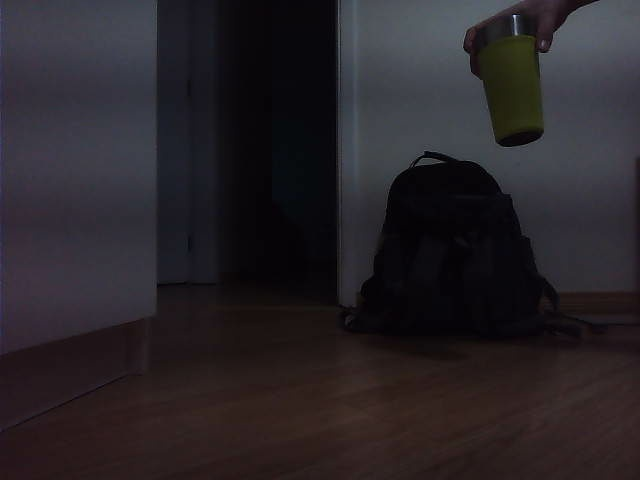
\includegraphics[width=\textwidth]{images/tg2/foto_para_calibrador.jpg}
    \caption{Imagem bruta capturada pela câmera do LIMO}
    \label{fig:foto_crua}
  \end{subfigure}

  \vspace{0.5cm} % Adiciona um espaço vertical entre as duas imagens

  % Segunda Imagem
  \begin{subfigure}[b]{1\textwidth}
    \centering
    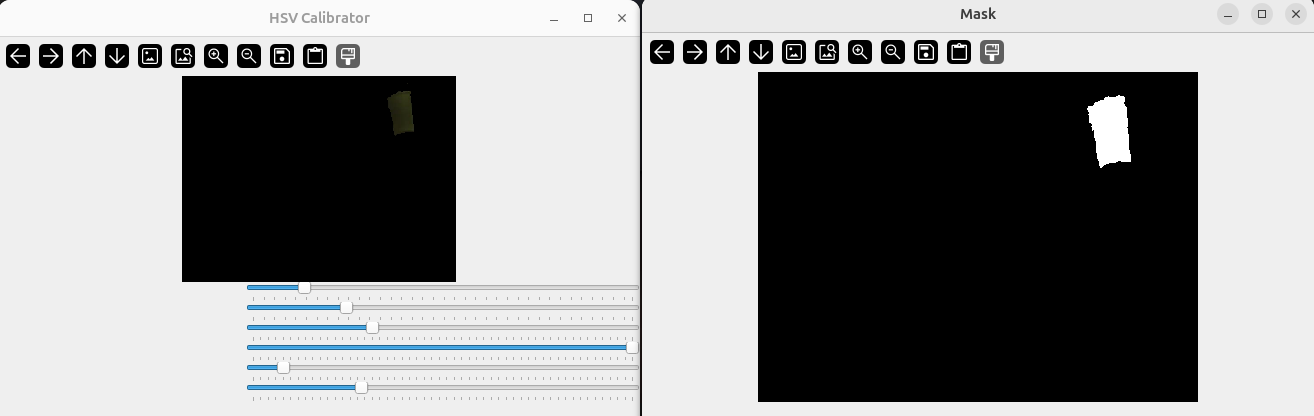
\includegraphics[width=\textwidth]{images/tg2/calibrador.png}
    \caption{Interface do calibrador HSV com máscara isolando o alvo}
    \label{fig:calibrador}
  \end{subfigure}

  \caption{Processo de calibração HSV para o alvo (copo verde neon).}
\end{figure}

\subsubsection{Nó 2 — \texttt{lidar\_reader}}

\textbf{Função:} dado o ângulo calculado pela câmera, retornar a distância
medida pelo LiDAR naquela direção.

\textbf{Subscreve:}
\begin{itemize}
  \item \texttt{/scan} (\texttt{sensor\_msgs/LaserScan}) — varredura contínua do LiDAR
  \item \texttt{/target/detection} — ângulo do alvo publicado pelo \texttt{color\_detector}
\end{itemize}

\textbf{Publica:} \texttt{/lidar/distance\_at\_angle} — vetor
\texttt{[angle\_deg, distance\_m, valid]}

\textbf{Método:} o ângulo em graus é convertido para o índice correspondente
no array de ranges do \texttt{LaserScan}. Para robustez, a distância é calculada
como a mediana de uma janela de 5 leituras vizinhas, descartando valores fora
dos limites válidos e leituras \texttt{NaN}/\texttt{Inf}.

\begin{table}[H]
\centering
\caption{Parâmetros de filtragem e leitura do sensor LiDAR.}
\label{tab:params_lidar}
\begin{tabular}{lp{9cm}}
\hline
\textbf{Parâmetro (Unidade)} & \textbf{Descrição detalhada} \\ \hline
Faixa Angular Válida (graus) & Define o campo de visão frontal considerado para busca (ex: $\pm$ 60° em relação ao eixo central). \\
Distância Mínima Válida (m) & Limite inferior para ignorar leituras muito próximas ao próprio corpo do robô ou ruídos. \\
Distância Máxima Válida (m) & Limite superior para desconsiderar objetos muito distantes que não fazem parte do cenário de interesse. \\ \hline
\end{tabular}
\end{table}

\subsubsection{Nó 3 — \texttt{sensor\_fusion}}

\textbf{Função:} combinar direção (câmera) e distância (LiDAR) em uma estimativa
suavizada da posição relativa do alvo, entregando ao controlador os erros prontos
para uso.

\textbf{Subscreve:}
\begin{itemize}
  \item \texttt{/target/detection}
  \item \texttt{/lidar/distance\_at\_angle}
\end{itemize}

\textbf{Publica:} \texttt{/target/pose} — vetor
\texttt{[found, angle\_deg, distance\_m, error\_angular\_norm, error\_distance\_m]}

\textbf{Método:} a fusão é geométrica e direta (\textit{feature-level fusion}).
Os valores brutos dos sensores são suavizados com um filtro exponencial:

\begin{equation}
  \label{eq:filtro}
  \hat{x}_t = \alpha \cdot x_t + (1 - \alpha) \cdot \hat{x}_{t-1}
\end{equation}

O erro angular normalizado $e_\theta \in [-1, 1]$ alimenta o controle de
rotação, e o erro de distância $e_d = d - d_{desejada}$ alimenta o controle
de avanço.

\begin{table}[H]
\centering
\caption{Parâmetros de configuração do nó de fusão sensorial.}
\label{tab:params_fusion}
\begin{tabular}{lp{9cm}}
\hline
\textbf{Parâmetro (Unidade)} & \textbf{Descrição detalhada} \\ \hline
Distância Alvo (m) & Valor de referência que o robô deve manter em relação ao objeto detectado. \\
\textit{Timeout} do Alvo (s) & Tempo máximo de persistência do dado de fusão antes de invalidar a posição. \\
Fator de Suavização Angular ($\alpha$) & Coeficiente do filtro passa-baixa para suavizar as variações bruscas no ângulo do alvo. \\
Fator de Suavização de Distância ($\alpha$) & Coeficiente aplicado para filtrar ruídos e saltos nas leituras de distância do LiDAR. \\ \hline
\end{tabular}
\end{table}

\subsubsection{Nó 4 — \texttt{follower\_controller}}

\textbf{Função:} converter os erros calculados pela fusão em comandos de
velocidade para o robô.

\textbf{Subscreve:} \texttt{/target/pose}

\textbf{Publica:} \texttt{/cmd\_vel} (\texttt{geometry\_msgs/Twist})

\textbf{Método:} controlador proporcional com três modos de
operação:

\begin{enumerate}
  \item \textbf{Seguimento normal} — alvo visível: rotação proporcional ao
  erro angular; avanço/recuo proporcional ao erro de distância (somente quando
  já alinhado).

  \item \textbf{Recovery behavior} — alvo perdido: o robô gira lentamente no
  último sentido em que viu o alvo, tentando reencontrá-lo por até
  \texttt{recovery\_timeout} segundos.

  \item \textbf{Parada de segurança} — se o tópico \texttt{/target/pose} parar
  de ser publicado por qualquer razão (falha de nó, etc.), um timer independente
  zera \texttt{/cmd\_vel} em até 0,5 s.
\end{enumerate}

\begin{equation}
  \label{eq:controlador}
  \omega = -K_{p,\omega} \cdot e_\theta \qquad
  v = K_{p,v} \cdot e_d \cdot \mathbf{1}_{|e_\theta| < 0{,}3}
\end{equation}


\begin{table}[H]
\centering
\caption{Parâmetros de configuração e controle do sistema de seguimento.}
\label{tab:params_controller}
\begin{tabular}{lp{9cm}}
\hline
\textbf{Parâmetro (Unidade)} & \textbf{Descrição detalhada do comportamento} \\ \hline
Ganho Angular ($K_p$) & Define a intensidade da correção de rotação para alinhar o robô ao centro do alvo. \\
Ganho Linear ($K_p$) & Define a velocidade de aproximação ou recuo baseada no erro de distância. \\
Velocidade Linear Máxima (m/s) & Limite superior de segurança para deslocamentos frontais e traseiros. \\
Velocidade Angular Máxima (rad/s) & Limite superior para a velocidade de rotação no próprio eixo. \\
Zona Morta Angular & Tolerância de erro de alinhamento para evitar oscilações constantes. \\
Zona Morta de Distância (m) & Faixa de tolerância em torno da distância alvo de 1 metro. \\
\textit{Timeout} de Segurança (s) & Intervalo máximo sem detecção antes da interrupção total dos motores (\textit{E-stop}). \\
Velocidade de Recuperação (rad/s) & Velocidade constante aplicada para busca ativa em 360° após a perda do alvo. \\
\textit{Timeout} de Busca (s) & Tempo limite para o comportamento de rotação antes de retornar ao estado de repouso. \\ \hline
\end{tabular}
\end{table}

% --------------------------------------------------------------
\subsection{Modo 2 — Tarefas com Detecção YOLO}
\label{sec:modo2}
% --------------------------------------------------------------

O Modo 2 substitui a detecção por cor por detecção de objetos por categoria,
usando a rede YOLO, e introduz uma camada de execução de tarefas. Em vez de um
único comportamento de seguimento contínuo, o robô passa a executar sequências de
\textbf{ações primitivas} (girar, avançar, procurar, aproximar-se, alertar),
descritas em uma lista JSON. Essa organização prepara o sistema para, futuramente,
receber comandos em linguagem natural traduzidos por um modelo de linguagem, mas
já é plenamente funcional recebendo a lista de ações diretamente. A arquitetura é
ilustrada na Figura~\ref{fig:pipeline_yolo}.

\begin{figure}[H]
\centering
\resizebox{\textwidth}{!}{
\begin{tikzpicture}[
  node distance=1.3cm and 2.2cm,
  box/.style={rectangle, rounded corners, draw=gray!70, fill=gray!10,
              minimum width=2.7cm, minimum height=0.85cm, align=center,
              font=\small},
  sensor/.style={box, fill=blue!10, draw=blue!40},
  lib/.style={box, fill=green!12, draw=green!45},
  % labels de tópico com fundo branco: "mascaram" a seta e ficam legíveis
  topic/.style={font=\ttfamily\scriptsize, text=gray!55,
                fill=white, inner sep=1.5pt},
  arr/.style={-{Stealth}, thick, gray!80}
]

% Coluna 1 — sensores
\node[sensor] (cam) {Câmera RGB};
\node[sensor, below=of cam] (lid) {LiDAR};
\node[sensor, below=of lid] (odo) {Odometria};

% Coluna 2 — percepção
\node[box, right=of cam] (yolo) {\texttt{yolo\_detector}};
\node[box, right=of lid] (lrd)  {\texttt{lidar\_reader}};

% Coluna 3 — executor (mais à direita, na linha do LiDAR)
\node[box, right=3.2cm of lrd] (exec) {\texttt{task\_executor}};
\node[box, above=of exec] (act)  {\texttt{/task/actions}};

% Primitivas e robô: bem abaixo, para o /odom não cruzá-los
\node[lib, below=2.2cm of exec] (prim) {\texttt{robot\_primitives}};
\node[sensor, right=of prim] (rob) {Limo (\texttt{/cmd\_vel})};

% Conexões da percepção
\draw[arr] (cam) -- (yolo);
\draw[arr] (lid) -- (lrd);

% yolo_detector -> executor (desce pelo topo-esquerdo)
\draw[arr] (yolo.east) -- ++(0.9,0) |- (exec.155)
    node[topic, pos=0.72]{/yolo/detection};

% lidar_reader -> executor (reto)
\draw[arr] (lrd) -- (exec)
    node[topic, midway]{/distance\_at\_angle};

% LiDAR bruto /scan -> executor (contorna por baixo do lidar_reader)
\draw[arr] (lid.south) -- ++(0,-0.45) -| (exec.205)
    node[topic, pos=0.30]{/scan};

% Odometria -> executor (entra pela base-esquerda)
\draw[arr] (odo.east) -| (exec.250)
    node[topic, pos=0.30]{/odom};

% Entrada de ações e saída de comando
\draw[arr] (act) -- (exec);
\draw[arr] (exec) -- (prim);
\draw[arr] (prim) -- (rob);

\end{tikzpicture}
}
\caption{Arquitetura do modo de tarefas: percepção por YOLO, leitura do LiDAR e
odometria alimentam o \texttt{task\_executor}, que aciona as primitivas de
movimento em \texttt{robot\_primitives}.}
\label{fig:pipeline_yolo}
\end{figure}

\subsubsection{Nó — \texttt{yolo\_detector}}

\textbf{Função:} detectar objetos de uma classe-alvo na imagem da câmera e
calcular o ângulo horizontal do objeto em relação ao centro da imagem.

\textbf{Subscreve:} \texttt{/camera/rgb/image\_raw} (\texttt{sensor\_msgs/Image})

\textbf{Publica:}
\begin{itemize}
  \item \texttt{/yolo/detection} — vetor \texttt{[found, cx\_norm, cy\_norm, area, angle\_deg]}, no mesmo formato de \texttt{/target/detection} do Modo 1
  \item \texttt{/yolo/class} — \texttt{String} com a classe detectada
  \item \texttt{/yolo/image\_debug} — imagem anotada com a \textit{bounding box}
\end{itemize}

\textbf{Método:} a rede YOLOv3-tiny é carregada em formato \textit{darknet} com a
função \texttt{readNetFromDarknet} (módulo \texttt{cv2.dnn}). Cada quadro é
convertido em um \textit{blob}
$416 \times 416$ e submetido à rede; as saídas passam por filtragem por limiar de
confiança e por supressão não-máxima (NMS) para eliminar detecções redundantes.
A detecção de maior confiança da classe-alvo é convertida em ângulo pela mesma
relação geométrica do Modo 1, aproveitando o campo de visão da câmera. Como a
saída segue o formato do \texttt{color\_detector}, o \texttt{lidar\_reader} pode
ser reutilizado sem alteração de código — apenas com o remapeamento de
\texttt{/target/detection} para \texttt{/yolo/detection}.

\begin{table}[H]
\centering
\caption{Parâmetros de configuração do detector YOLO.}
\label{tab:params_yolo}
\begin{tabular}{lp{9cm}}
\hline
\textbf{Parâmetro (Unidade)} & \textbf{Descrição detalhada} \\ \hline
Classe Alvo & Categoria do dataset COCO a ser monitorada (ex.: \textit{sports ball}, \textit{person}, \textit{laptop}). \\
Limiar de Confiança & Confiança mínima para aceitar uma detecção; filtra predições fracas. \\
Limiar de NMS & Limiar de IoU usado na supressão não-máxima para descartar caixas sobrepostas. \\
HFOV da Câmera (graus) & Campo de visão horizontal, usado para converter a posição do objeto em ângulo. \\ \hline
\end{tabular}
\end{table}

\subsubsection{Nó — \texttt{task\_executor}}

\textbf{Função:} manter o estado dos sensores atualizado e executar, em sequência,
a lista de ações recebida.

\textbf{Subscreve:}
\begin{itemize}
  \item \texttt{/yolo/detection} e \texttt{/yolo/class} — percepção visual
  \item \texttt{/lidar/distance\_at\_angle} — distância ao alvo detectado
  \item \texttt{/scan} (\texttt{sensor\_msgs/LaserScan}) — LiDAR bruto, para o freio de segurança
  \item \texttt{/odom} (\texttt{nav\_msgs/Odometry}) — odometria das rodas
  \item \texttt{/task/actions} (\texttt{String} com JSON) — lista de ações a executar
\end{itemize}

\textbf{Publica:} \texttt{/cmd\_vel}, \texttt{/task/status} (estado atual: \texttt{IDLE},
\texttt{RUNNING: <ação>}, \texttt{ERROR: ...}) e \texttt{/task/alert}.

\textbf{Método:} os \textit{callbacks} dos sensores mantêm um objeto de estado
(\texttt{RobotState}) sempre atualizado. Ao receber uma lista de ações, o executor
valida o JSON e itera sobre cada ação, chamando a primitiva correspondente da
biblioteca \texttt{robot\_primitives} e publicando o status a cada etapa. Uma ação
especial \texttt{cancel} interrompe a sequência. A partir do \texttt{/scan} bruto,
o nó calcula continuamente a distância mínima no setor frontal de
$\pm 30°$, valor central para o freio de segurança e para os campos potenciais.

\subsubsection{Biblioteca \texttt{robot\_primitives}}

Diferentemente dos nós anteriores, \texttt{robot\_primitives} não é um nó ROS, mas
uma biblioteca importada pelo \texttt{task\_executor}. Cada primitiva é uma função
bloqueante que só retorna quando a ação termina ou o \textit{timeout} estoura. A
Tabela~\ref{tab:primitivas} resume as ações disponíveis.

\begin{table}[H]
\centering
\caption{Ações primitivas disponíveis no modo de tarefas.}
\label{tab:primitivas}
\begin{tabular}{lp{8.5cm}}
\hline
\textbf{Ação} & \textbf{Descrição} \\ \hline
\texttt{go\_forward} & Avança uma distância dada; usa odometria se disponível e para se o freio de segurança disparar. \\
\texttt{rotate} & Gira um ângulo dado (positivo = esquerda); acumula ângulo via odometria para suportar rotações maiores que 360°. \\
\texttt{scan\_area} & Rotação de 360° para varrer o ambiente. \\
\texttt{search\_object} & Gira lentamente até encontrar a classe-alvo via YOLO ou atingir o \textit{timeout}. \\
\texttt{approach\_object} & Aproxima-se do objeto com controle proporcional no ângulo e campos potenciais na velocidade linear. \\
\texttt{stop} & Interrompe o movimento imediatamente. \\
\texttt{alert} & Registra uma mensagem e a publica em \texttt{/task/alert}. \\ \hline
\end{tabular}
\end{table}

\subsubsection{Freio de Segurança}

O freio de segurança está ativo nas primitivas \texttt{go\_forward} e
\texttt{approach\_object}. A cada iteração do laço de controle, verifica-se a
distância mínima frontal medida pelo LiDAR; se ela cair abaixo de um limiar de
segurança $d_{\text{seg}}$, o robô é imediatamente parado e a ação é abortada:

\begin{equation}
  \label{eq:freio}
  d_{\text{frontal}} < d_{\text{seg}} \;\Rightarrow\; v = 0 .
\end{equation}

Neste projeto adotou-se $d_{\text{seg}} = 0{,}20$~m. O mecanismo é independente da
percepção visual, funcionando como uma camada de proteção mesmo que o YOLO falhe
em detectar um obstáculo.

\subsubsection{Campos Potenciais na Aproximação}

A primitiva \texttt{approach\_object} aplica a formulação de campos potenciais
apresentada na Seção~\ref{sec:campos} para regular a velocidade linear. A força
atrativa é proporcional ao erro entre a distância medida pelo LiDAR e a distância
desejada, e a força repulsiva atua quando um obstáculo entra no raio de
influência $d_0$. A velocidade angular, por sua vez, segue um controle
proporcional ao erro angular fornecido pelo YOLO ($e_\theta = c_{x,\text{norm}}$):

\begin{equation}
  \label{eq:aproximacao}
  \begin{aligned}
    \omega &= -k_{p,\omega}\, e_\theta, \\[1.5ex]
    v &= \underbrace{k_{p}\,(d - d_{\text{alvo}})}_{f_{\text{att}}}
       - \underbrace{k_{R}\!\left(\dfrac{1}{d} - \dfrac{1}{d_0}\right)}_{f_{\text{rep}},\; d < d_0} .
  \end{aligned}
\end{equation}

Ambas as velocidades são saturadas por limites máximos de segurança. A
Tabela~\ref{tab:params_approach} lista os valores adotados.

\begin{table}[H]
\centering
\caption{Parâmetros da aproximação por campos potenciais.}
\label{tab:params_approach}
\begin{tabular}{llp{6.5cm}}
\hline
\textbf{Parâmetro} & \textbf{Valor} & \textbf{Descrição} \\ \hline
$k_{p}$ (ganho atrativo)        & 0,40 & Intensidade da força de atração ao alvo. \\
$k_{R}$ (ganho repulsivo)       & 0,15 & Intensidade da força de repulsão de obstáculos. \\
$d_0$ (raio de influência)      & 0,50~m & Distância a partir da qual a repulsão passa a atuar. \\
$d_{\text{seg}}$ (freio)        & 0,20~m & Distância mínima frontal antes da parada de emergência. \\
$k_{p,\omega}$ (ganho angular)  & 0,60 & Ganho do controle proporcional de rotação. \\ \hline
\end{tabular}
\end{table}

\subsubsection{Odometria}

As primitivas \texttt{go\_forward} e \texttt{rotate} utilizam o tópico
\texttt{/odom} para medir deslocamento e rotação reais a partir dos
\textit{encoders} das rodas. O ângulo de guinada (\textit{yaw}) é extraído
diretamente do quatérnion de orientação, sem dependência da biblioteca \textit{tf}:

\begin{equation}
  \label{eq:yaw}
  \psi = \operatorname{atan2}\!\big(2(q_w q_z + q_x q_y),\; 1 - 2(q_y^2 + q_z^2)\big) .
\end{equation}

Quando a odometria não está disponível (tópico silencioso), as primitivas
retornam automaticamente à estimativa por tempo, sem necessidade de configuração
manual, garantindo robustez do sistema.


% ══════════════════════════════════════════════════════════════
\newpage
\section{Resultados Experimentais}
% ══════════════════════════════════════════════════════════════

% --------------------------------------------------------------
\subsection{Seguimento por Cor (Fusão Sensorial)}
% --------------------------------------------------------------

\subsubsection{Detecção Visual do Alvo}

A detecção por segmentação HSV foi validada com sucesso. A
Figura~\ref{fig:follower} mostra o sistema em operação: o alvo (copo verde neon)
é identificado corretamente, com \textit{bounding box} verde delimitando o objeto,
indicação do ângulo calculado e o texto de detecção ativa.

\begin{figure}[H]
  \centering
  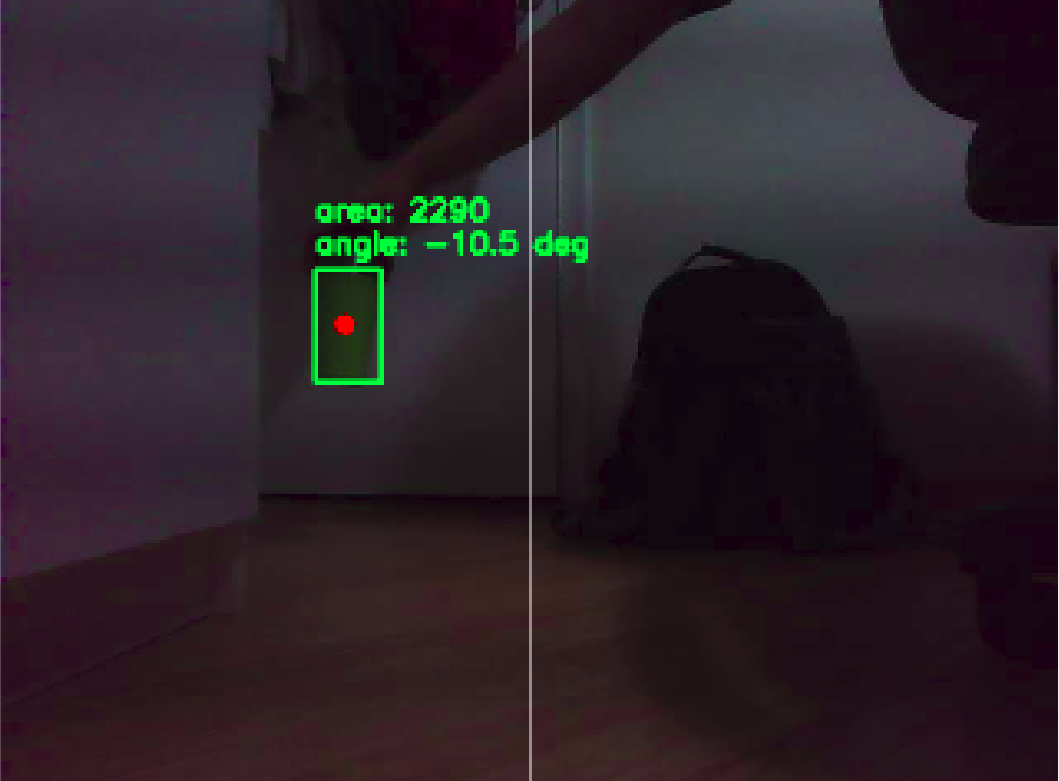
\includegraphics[width=0.7\textwidth]{images/tg2/follower.png}
  \caption{Sistema de detecção em operação: \textit{bounding box} verde em volta
  do copo com ângulo calculado exibido em tempo real.}
  \label{fig:follower}
\end{figure}

\subsubsection{Fusão de Sensores}

A fusão câmera + LiDAR foi validada com o nó \texttt{sensor\_fusion} ativo.
O trecho de log abaixo mostra a consistência dos dados dos dois sensores operando
em conjunto:

\begin{lstlisting}[caption={Log do sistema com fusão ativa},
                   basicstyle=\footnotesize\ttfamily, breaklines=true]
[INFO]: Alvo detectado | angle=12.8 deg | cx_norm=0.42 | area=2714
[INFO]: LiDAR | angulo=12.8 deg | dist=3.04 m
[INFO]: Fusao | ang=12.9 deg | dist=3.07 m | err_ang=0.43 | err_dist=2.07 m
\end{lstlisting}

A câmera e o LiDAR concordam no ângulo ($12{,}8°$) e o LiDAR fornece a
distância métrica ($3{,}04$ m). O erro de distância de $2{,}07$ m indica que o
alvo estava a $\approx 3$ m enquanto a distância desejada é $1$ m —
comportamento correto e esperado.

\subsubsection{Seguimento Autônomo}

O sistema completo foi executado com sucesso. O robô
demonstrou capacidade de seguir o alvo de forma contínua, mantendo a distância
configurada de 1 metro e realizando rotação proporcional ao desvio angular. O
comportamento de recuperação (\textit{recovery behavior}) também foi observado:
ao perder o alvo de vista, o robô gira lentamente no último sentido detectado
até reencontrá-lo ou atingir o timeout de 4 segundos.

% --------------------------------------------------------------
\subsection{Detecção por YOLO}
% --------------------------------------------------------------

A detecção de objetos por categoria foi validada com o nó \texttt{yolo\_detector}
executando o modelo YOLOv3-tiny a bordo do LIMO. A Figura~\ref{fig:yolo_laptop}
mostra o sistema em operação, detectando corretamente um \textit{laptop}: a
\textit{bounding box} verde delimita o objeto, o ponto vermelho marca seu centro e
o rótulo exibe a classe, a confiança da detecção ($46\%$) e o ângulo horizontal
estimado em relação ao centro da imagem ($3{,}3°$), próximo de zero por o objeto
estar quase centralizado.

\begin{figure}[H]
  \centering
  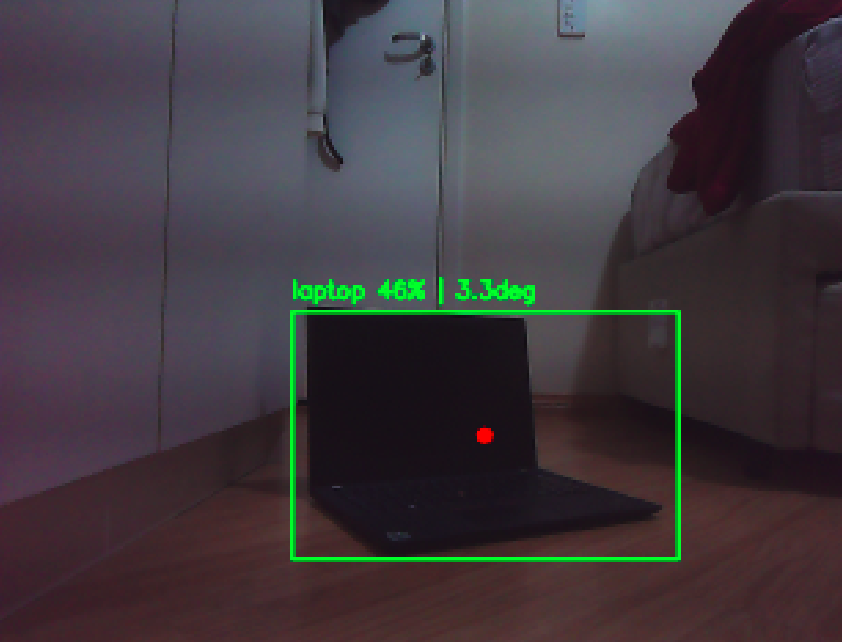
\includegraphics[width=0.7\textwidth]{images/tg2/laptop_yolo.png}
  \caption{Detecção de um \textit{laptop} pelo YOLOv3-tiny: \textit{bounding box},
  centro do objeto, classe, confiança e ângulo calculado exibidos em tempo real.}
  \label{fig:yolo_laptop}
\end{figure}

Observou-se que a qualidade das detecções é sensível às condições de iluminação
do ambiente: em cenas com pouca luz, a confiança das predições cai e algumas
classes tornam-se mais difíceis de detectar de forma estável. Esse comportamento
é coerente com o uso da variante \textit{tiny} da rede, que troca parte da
precisão por velocidade de inferência para viabilizar a execução na Jetson Nano.

% --------------------------------------------------------------
\subsection{Aproximação com Campos Potenciais}
% --------------------------------------------------------------
% TODO: escrever (depende de teste no robô). Incluir os gráficos gerados pelo
% plot_task.py a partir do CSV do task_logger: distância ao alvo, LiDAR mínimo
% frontal, forças atrativa/repulsiva, cmd_vel, ângulo YOLO e trajetória XY.
\textit{[Seção a ser escrita.]}


% ══════════════════════════════════════════════════════════════
\newpage
\section{Conclusão}
% ══════════════════════════════════════════════════════════════
% TODO: reescrever como conclusão final (hoje é conclusão parcial).
% Retomar: os dois modos implementados e validados em hardware real; o que a
% fusão sensorial e os campos potenciais agregaram; limitações observadas
% (iluminação, LiDAR sem visão traseira); e perspectivas futuras.
\textit{[Seção a ser escrita.]}

% ----- Conteúdo da versão parcial preservado abaixo (comentado) -----
% O sistema de seguimento de alvo visual com fusão de sensores foi implementado e
% validado em hardware real. Os quatro nós do pipeline operam de forma integrada,
% com comunicação via tópicos ROS, parâmetros configuráveis externamente e
% comportamentos de segurança implementados.
%
% \subsection{Cronograma}
% (lista de próximos passos da versão parcial — não se aplica ao relatório final)
